%! Mode:: "TeX:UTF-8"
%! TEX program = xelatex
\PassOptionsToPackage{quiet}{xeCJK}
\documentclass[withoutpreface,bwprint]{cumcmthesis}
\usepackage{etoolbox}
\BeforeBeginEnvironment{tabular}{\zihao{-5}}
\usepackage[framemethod=TikZ]{mdframed}  % 框架宏包
\usepackage{url}  % 网页链接宏包
\usepackage{setspace}
\usepackage{graphicx}
%%%%%%%%%%%%%%%%%%%%%%%%%%%%%%%%%%%%%%%%%%%%%%%%%%%%%%%%
%下面是美赛搬过来的usepackage
\usepackage{pgfplots}
\pgfplotsset{compat=1.18}
%\usepackage{palatino}  % 帕拉提诺体字体宏包
%\usepackage{times}  % 正文使用Times New Roman风格字体
%\usepackage{newtxmath}
\usepackage{lipsum}  % 导入生成段落的宏包
\usepackage{indentfirst}
\usepackage{booktabs} % For professional-looking tables
\usepackage{xcolor}   % For cell coloring
\usepackage{colortbl} % Required for \rowcolor
\definecolor{LightGreen}{rgb}{0.9, 0.95, 0.9}
\definecolor{LightBlue}{RGB}{229, 238, 255}
\definecolor{LightPink}{RGB}{255, 229, 237}
\usepackage{fancyhdr}
\usepackage{enumitem} % 用于自定义列表格式
\usepackage{setspace}
\usepackage{booktabs}  % 三线表加粗
\usepackage{float}
\usepackage{eso-pic}  % 用于在页面添加背景
\usepackage{graphicx} % 图片支持
\usepackage{tikz}     % 用于绘制半透明覆盖层
\usepackage{subcaption}
\usepackage{caption}
\setlist[itemize]{listparindent=2em}
\setlist[enumerate]{listparindent=2em}
\usepackage[titles]{tocloft}
\usepackage{tabularx}
\usepackage[titles]{tocloft}
\setlength{\cftbeforesecskip}{8pt}   % 节前间距
\setlength{\cftbeforesubsecskip}{4pt} % 小节前间距
\urlstyle{rm}
\setlength{\headheight}{13.6pt}
\lstset{
    basicstyle=\footnotesize\ttfamily, % 字体大小和类型
    numbers=left,               % 在左侧显示行号
    numberstyle=\tiny,          % 设置行号字体
    numbersep=5pt,              % 行号与代码间距
    showspaces=false,           % 不显示空格
    showstringspaces=false,     % 字符串中不显示空格
    showtabs=false,             % 不显示制表符
    tabsize=2,                  % 制表符大小
    breaklines=true,            % 自动换行
    breakatwhitespace=false,    % 只在空格处换行
    title=\lstname,             % 显示文件名
    escapeinside={\%*}{*)},     % LaTeX代码嵌入
    xleftmargin=10pt,           % 左边距
    xrightmargin=10pt,          % 右边距
    aboveskip=5pt,              % 上方间距
    belowskip=5pt,              % 下方间距
    lineskip=-1pt               % 减小行距（负值可以压缩行距）
}
\newcolumntype{C}{>{\centering\arraybackslash}X}
\newcolumntype{R}{>{\raggedleft\arraybackslash}X}
\newcolumntype{L}{>{\raggedright\arraybackslash}X}
\renewcommand{\abstractname}{摘\kern1em要}
\title{NIPT时点选择与孕妇风险和胎儿状态异常分析}  % 论文标题
\tihao{}  % 题号
\baominghao{}  % 报名号
\schoolname{}  % 学校
\membera{}  % 队员a
\memberb{}  % 队员b
\memberc{}  % 队员c
\supervisor{}  % 指导老师
\yearinput{}
\monthinput{}
\dayinput{}

%%%%%%%%%%%%%%%%%%%%%%%%%%%%%%%%%%%%%%%%%%%%%%%%%%%%%%%%%%%%%
%% 正文
\begin{document}

\maketitle
\begin{abstract}
\indent 在产前筛查、产前诊断的工作需求水平不断提高的大环境下，为了降低出生缺陷发生率，减少唐氏综合症等畸形胎儿主要出现的问题，发展无创产前检测技术处在核心地位。依据某地孕妇的无创产前检测技术（NIPT）数据的实际情况，本文主要研究回应对不同人群NIPT时点选择的分组策略以及各组中的最佳的NIPT时点，不同因素对男胎Y染色体浓度增长模式的关联关系，女胎状态的判定方法。通过\textbf{线性混合效应模型}、\textbf{Pearson相关系数矩阵}、\textbf{改进的Canopy-Kmeans算法}等进行求解。\\\indent
\textbf{针对问题一}:进行数据处理，将孕周数转换为小数形式，把孕周数与BMI分别与胎儿Y染色体浓度使用\textbf{Pearson相关系数矩阵分析}，并进行\textbf{相关热力图可视化}。通过\textbf{混合线性回归}，求解出孕周数与胎儿Y染色体浓度、BMI与胎儿Y染色体浓度的关系模型，最后使用\textbf{Pearson相关系数检验}说明了关系的显著性。最终求解结果为\( YC_{ij} = 0.0031W_{ij}-0.0014BMI_{ij} + \gamma_i + \varepsilon_{ij} + 0.0697\)。

\textbf{针对问题二}:首先进行数据提取，记录每位孕妇测量胎儿Y染色体浓度首次达到4\%的时点进一步处理，通过改进的 \textbf{Canopy-Kmeans算法} 对其进行聚类分组，随后构造一个包含检测有效性、安全性的风险函数，使用\textbf{熵权法}确定风险函数权重，函数表达式为\(R = 0.3435(1 - p) + 0.6565T(t)\)，利用遍历算法最小化风险值求解测量的最佳时点。最后进行 BMI 方差检验与误差分析，分析理论最佳时点的前后两周的风险变化。

\textbf{针对问题三}:与问题二类似，主要考虑 BMI 对男胎 Y 染色体浓度的影响，同时把身高、体重、年龄纳入综合考虑因素，利用\textbf{线性混合效应模型}拟合多因素与男胎 Y 染色体浓度的关系。由于改进的Canopy-Kmeans算法在综合考虑因素时粗聚类过程中容易分组过多，本问采用 \textbf{\textit{K}-means} 算法对其进行聚类分组。构造\textbf{风险函数}，通过相关性系数与显著性检验确定权重，表达式为\(R = 0.30915(1 - p) + 0.59085T(t) + 0.1w\)最终通过遍历算法最小化风险值求解测量的最佳时间，与问题二同样进行 BMI 方差检验与误差分析。

\textbf{针对问题四}:为便于分别预测三条染色体数目异常的诱因，将附件中的数据按染色体类别拆分，并将每条染色体的状态转化为 \textbf{0-1} 变量：拷贝数正常记为 0，存在非整倍性则记为 1。再将检测孕周、孕妇 BMI、测序读段数、GC 含量、Z 值、X 染色体浓度以及经\textbf{二值化编码}的常染色体非整倍性状态作为特征，利用决策树模型的 \textbf{CART算法} 进行训练。通过计算各特征的重要性，只要有一条染色体异常概率$> 0.5$，则判定为胎儿状态异常，根据该规则构建对女胎异常的预测模型，具体预测结果与实际结果对比见文件：详细预测结果与实际结果分析.xlsx。特别地，通过训练得到的决策树模型，可构建一个交互式判定程序。用户输入相关指标值后，即可直接获取女胎是否异常的判定结果。



\keywords{线性混合效应模型~~Pearson相关系数~~热力图~~Canopy-Kmeans~~熵权法~~CART}
\end{abstract}
%%%%%%%%%%%%%%%%%%%%%%%%%%%%%%%%%%%%%%%%%%%%%%%%%%%%%%%%%%%%% 

% \tableofcontents  % 目录
% \newpage

%%%%%%%%%%%%%%%%%%%%%%%%%%%%%%%%%%%%%%%%%%%%%%%%%%%%%%%%%%%%%  
\section{问题重述}
\subsection{问题背景}
\vspace{-5pt}2013年统计结果显示，我国出生缺陷发生率约为5.6\%，属于生育缺陷高发国，为了控制和预防出生缺陷\upcite{1}，使得公民更加充分地行使自由生育的权利，亟需加强产前检测技术，确保胎儿的顺利产出\upcite{2}。现研究无创产前检测技术（NIPT）检测胎儿状态，可以检测胎儿是否畸形，预防唐氏综合症等畸形胎儿主要出现的问题。21号、18号和13号染色体的浓度是检测畸形的决定性标准，胎儿性染色体浓度是验证NIPT的准确性的重要标准。NIPT检测分为男胎检测和女胎检测，由于男胎含有Y染色体，女胎不含Y染色体，男胎的NIPT检测判定稍为容易，为首先需要研究的问题。由实践表明，胎儿性染色体浓度可在孕期的10周至25周进行NIPT检测，越早检测风险越低，在12周以内发现风险较低，需要控制检测时间在12周以内。对于男胎NIPT检测，若男胎Y染色体浓度$\geq4\%$，则可认为NIPT检测结果可信。注意到，男胎Y染色体浓度与怀孕周数和孕妇的BMI值有重要关系，需要根据孕妇的BMI值分组，划分不同BMI范围的孕妇的最佳NIPT检测时点（即Y染色体浓度$\geq4\%$）。在检测过程中可能会出现因检测时点等而引发的测序失败的问题，另外，孕妇可能需要多次采血或多次检测来提高检测信度。
%%%%%%%%%%%%%%%%%%%%%%%%%%%%%%%%%%%%%%%%%%%%%%%%%%%%%%%%%%%%% 
\vspace{-13pt}\subsection{问题提出}

附件含某地孕妇的NIPT数据，包含：孕妇身高、体重、检测孕周、基因读段数、染色体浓度、染色体Z值等关键数据。现需结合当地实际情况与附件所给信息建立数学模型，分析以下问题：

\textbf{问题一}：由于胎儿Y染色体浓度是验证其NIPT检测的准确性的重要标准，而胎儿Y染色体浓度与孕妇的许多指标有关，要求分析胎儿Y染色体浓度与孕妇的怀孕时间和BMI值等数据的相关性，并检验相关指标的显著性。

\textbf{问题二}：由于孕妇BMI显著影响男胎Y染色体浓度上升情况，要求根据男胎孕妇的BMI指标进行区间分组，分别确定各组的最佳NIPT时间节点，最大化不同分组间染色体浓度增长模式的差异性、同一分组内染色体浓度增长模式的相似性，并分析给定的节点对于各组人群的误差。

\textbf{问题三}：在第二问的基础上，继续探究身高、体重等可能影响因素对男胎Y染色体浓度上升情况的影响，最小化孕妇潜在风险，制定更加个性化的分组和时点推荐方案。

\textbf{问题四}：男胎NIPT检测研究之后需要研究女胎的检测方案。由于女胎没有Y染色体，需要综合考虑女胎21号、18号和13号染色体对应的Z值、GC含量、读段数、BMI等因素制定女胎异常的判定策略。

%%%%%%%%%%%%%%%%%%%%%%%%%%%%%%%%%%%%%%%%%%%%%%%%%%%%%%%%%%%%% 

\section{问题分析}
\subsection{问题一分析}
\begin{figure}[ht]
\centering
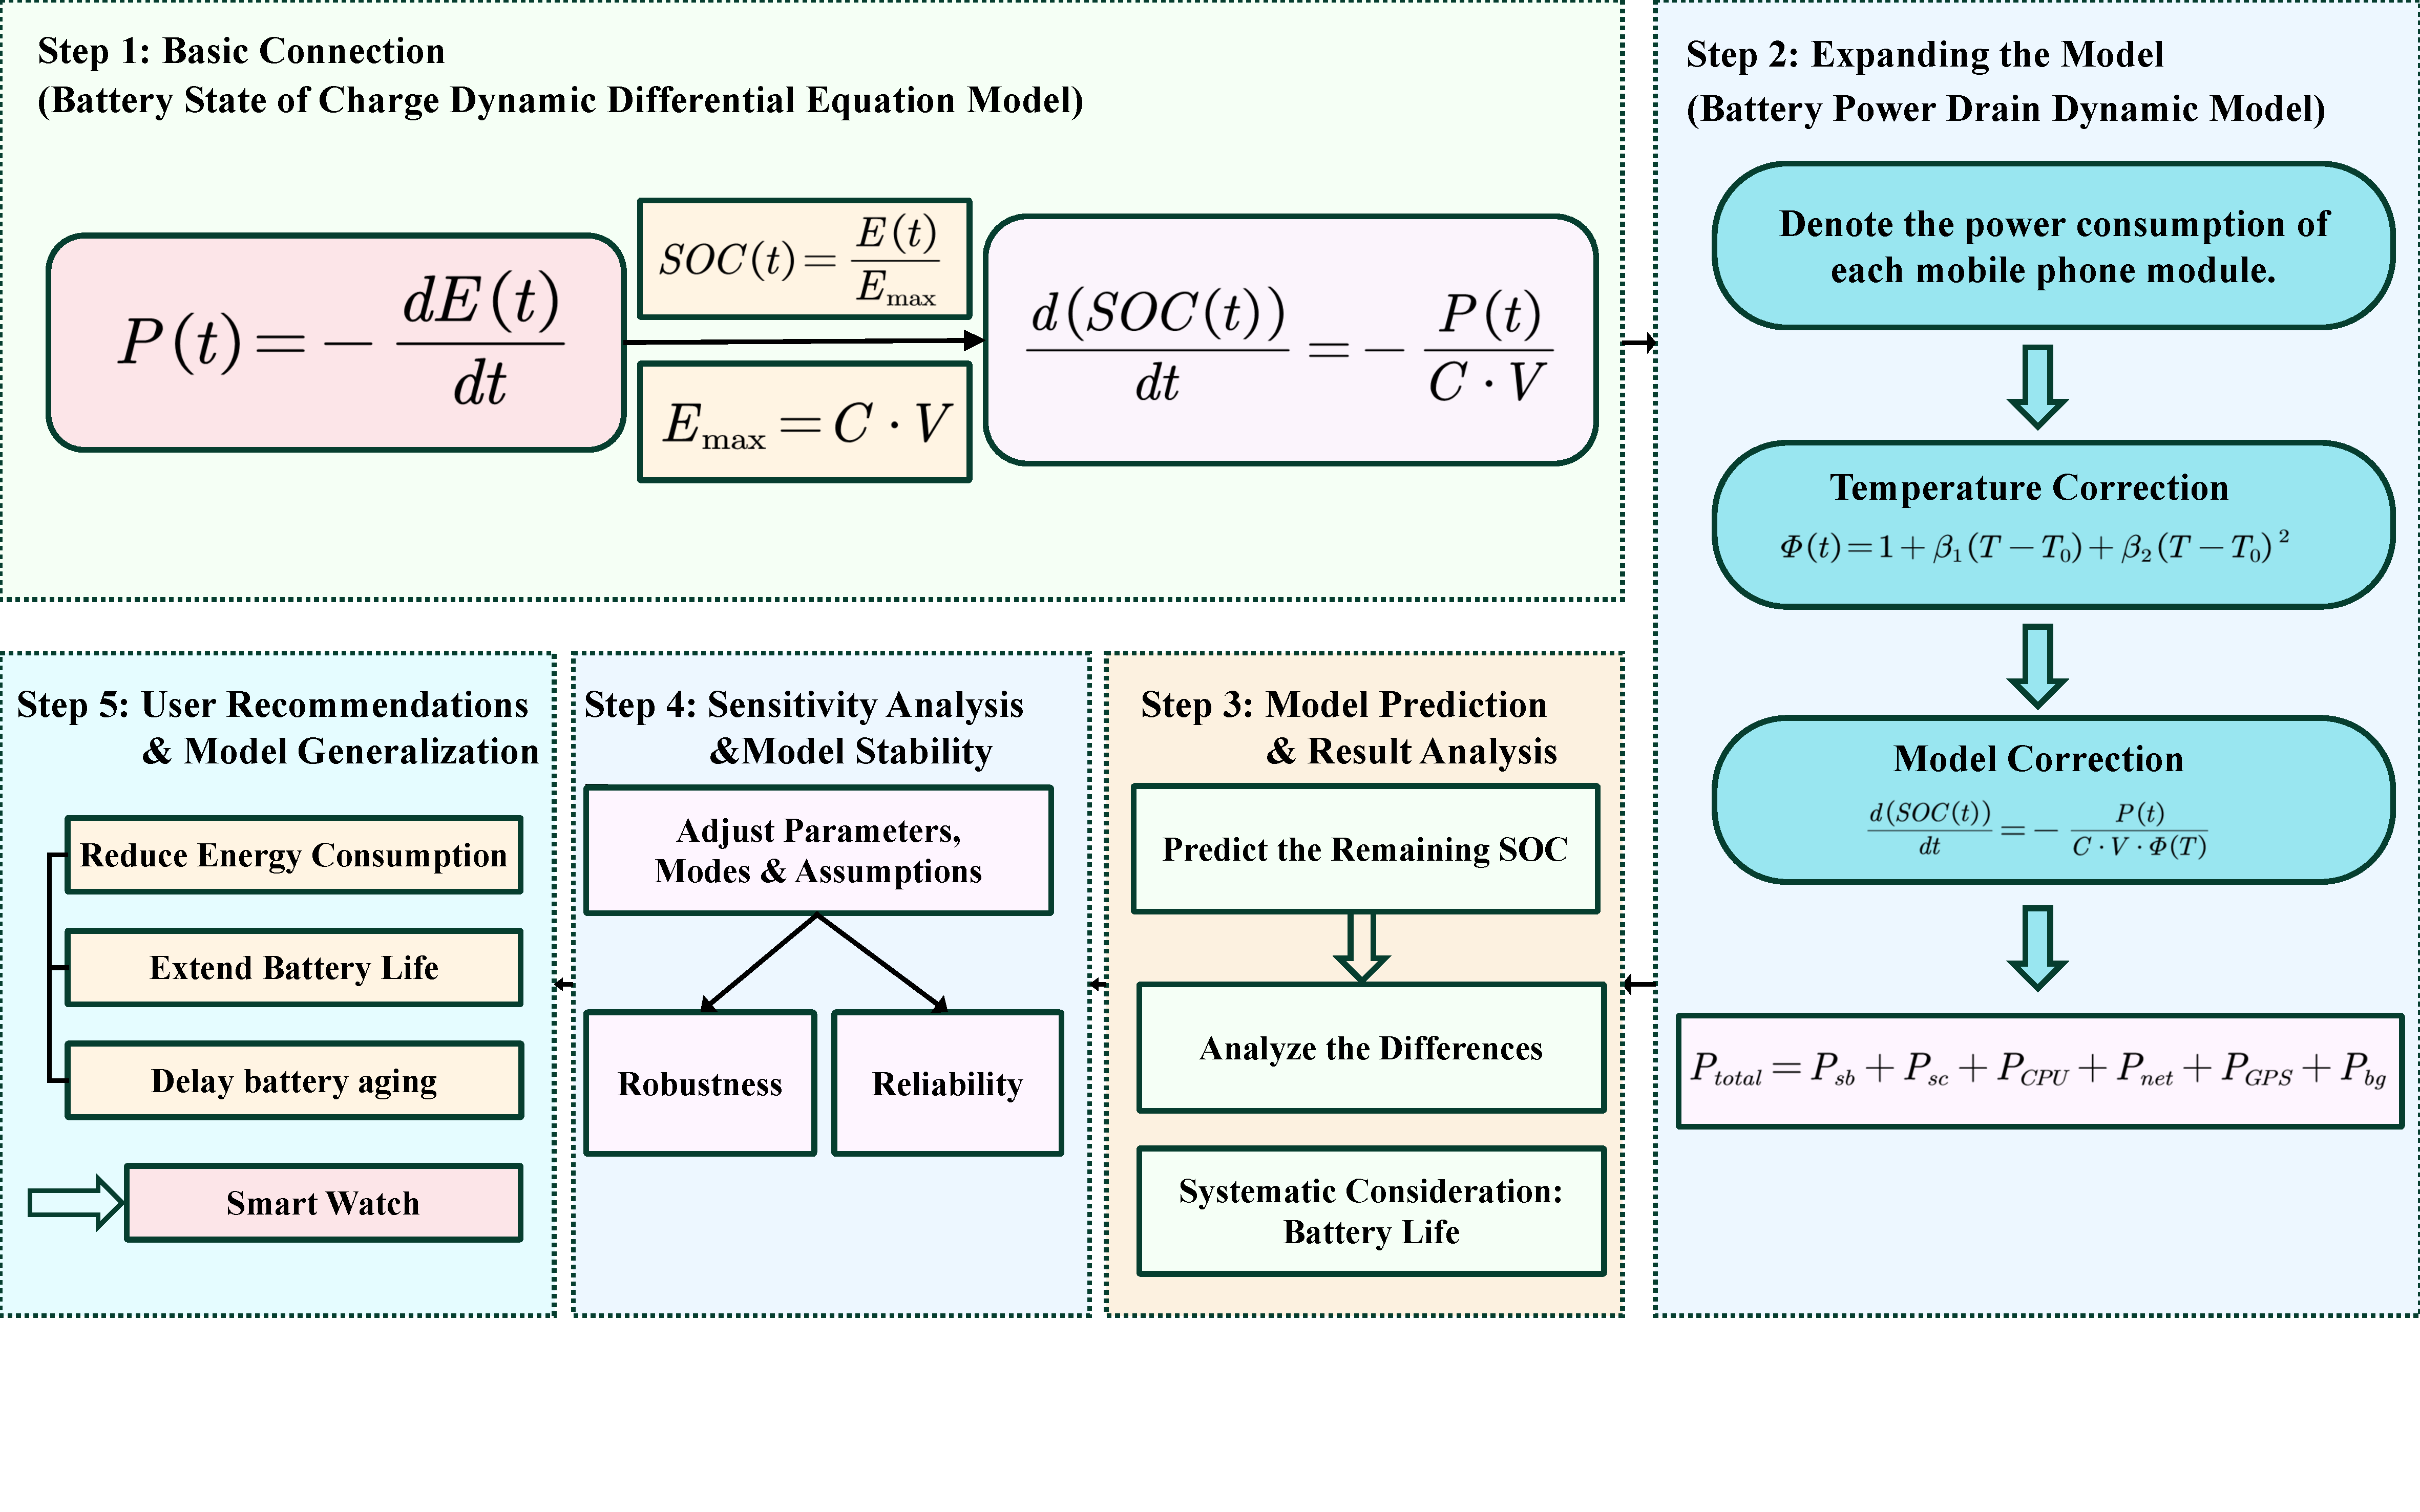
\includegraphics[width=1.05\textwidth,trim=0cm 6.5cm 0cm 0cm, 
clip]{figures/2026美赛流程图.pdf}
\caption{问题一分析流程图}
\label{fig:问题一分析}
\end{figure}
需要给出胎儿Y染色体浓度与孕周数和BMI的关系模型，若有其他与胎儿Y染色体浓度相关性较强的指标亦可分析。给出关系模型需要两个步骤，分析指标间的相关性并检验显著性、通过合适的回归方式求解关系方程。
首先进行数据处理，将孕周数转换为小数，精确量化孕周数，使得关系模型更加精确。
\begin{enumerate}[label=(\arabic*)]
    \item 分析指标间的相关性并检验显著性：将胎儿Y染色体浓度与题目给定的两个指标使用\textbf{Pearson相关系数矩阵}分析相关性并进行\textbf{热力图可视化}分析，并对其进行\textbf{Pearson相关系数检验}。
    \item 通过合适的回归方式求解关系方程：画出需要研究的两个指标间的散点图，首先可以考虑较为通用的线性回归模型进行拟合，若拟合效果较差，可考虑非线性拟合、多项式回归或指数回归等进行拟合。
\end{enumerate}


\subsection{问题二分析}	
\begin{figure}[ht]
\centering
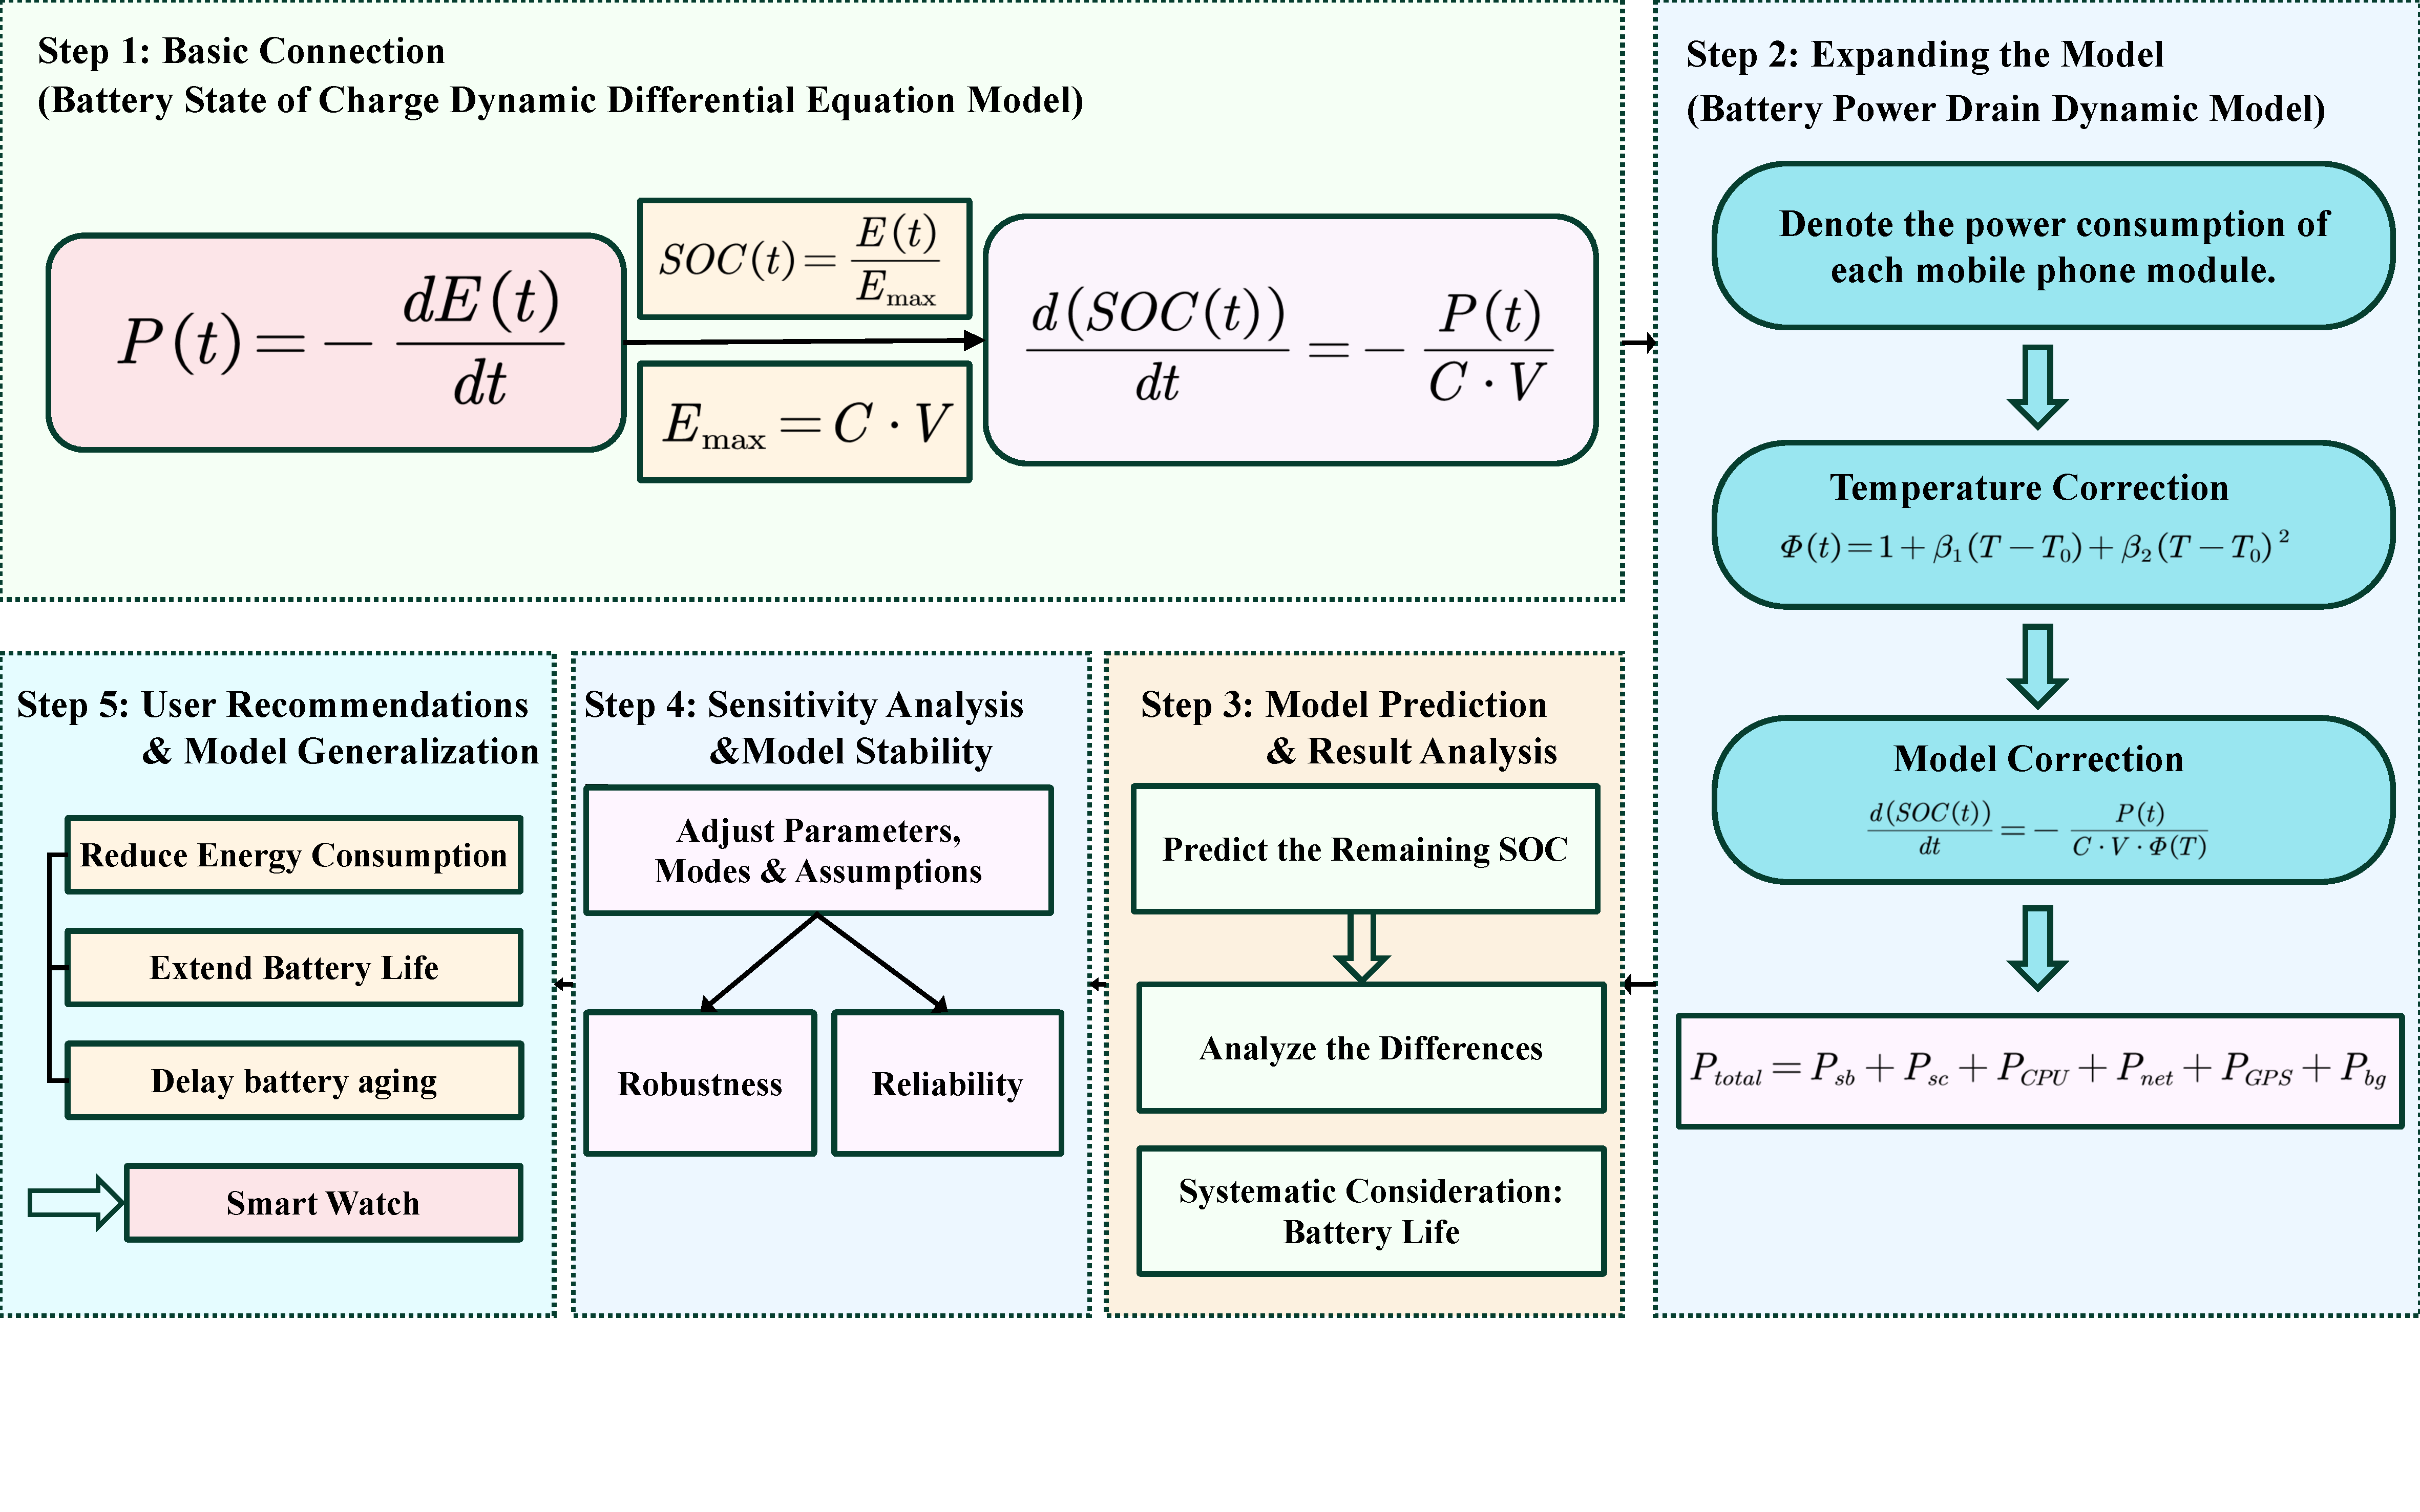
\includegraphics[width=1.05\textwidth,trim=0cm 6.5cm 0cm 0cm, 
clip]{figures/2026美赛流程图.pdf}
\caption{问题二分析流程图}
\label{fig:问题一分析}
\end{figure}

需要根据胎儿Y染色体浓度的最早达标时间对男胎孕妇的BMI进行分组，并给出每组的最佳NIPT时间节点，并分析给定的节点对于各组人群的误差。为了增加分组区间内NIPT时点的代表性，最大化不同分组间染色体浓度增长模式的差异性、同一分组内染色体浓度增长模式的相似性，聚类算法需具有良好的区分度，具体的算法步骤如下：

\textbf{Step 1.} 可以考虑\textbf{数据提取}，记录每位孕妇测量胎儿Y染色体浓度首次达到4\%的时点进一步处理

\textbf{Step 2.} 进行聚类分组，聚类模型可以考虑改进的\textbf{Canopy-Kmeans算法}

\textbf{Step 3.} 随构造一个包含检测时间、安全性的风险函数，风险函数包含有效性风险和安全性风险，有效性风险是孕妇检测时男胎Y染色体浓度是否达到4\%的风险，安全性风险是孕妇的胎儿随着检测时间的推移可治疗时间缩短的风险

\textbf{Step 4.} 最小化风险值求解测量的最佳时间

\textbf{Step 5.} 最后进行误差分析，对拟合效果进行检验，优化风险函数

\subsection{问题三分析}
题目要求研究多种指标对男胎Y染色体浓度的影响，可以综合问题一和问题二的模型，利用问题一建立的\textbf{线性混合效应模型}拟合多因素与男胎Y染色体浓度的关系，使用\textbf{K-means聚类}对孕妇群体分组，由于熵权法过于客观，可能不能满足现实需求，这一问需要通过相关性分析和相关性检验确定风险权重，随后细化问题二构造的\textbf{风险函数}，增加题目要求的指标，通过遍历算法最小化风险值求解测量的最佳时间，最后进行误差分析，对拟合效果进行检验，优化风险函数。

\subsection{问题四分析}
通过查阅文献得知可以将$|Z|>3$作为胎儿状态异常的初步判断标准\upcite{3}，但通过对题目所给数据分析，不能使用此标准直接形成最终的判断标准，因为通过数据筛选，染色体组的Z值满足$|Z|>3$的数据点较少，特别是对于18号染色体的Z值，不存在满足$|Z|>3$的个体。另外，附件大部分个体即使某染色体组的Z值满足$|Z|>3$的条件，也不存在染色体异常的情况，注意到序号为343，代码为B079的孕妇在20-21周测量的X染色体的Z值达到了10.29，但对于13、18和21号染色体，均未发现非整倍体异常，于是考虑使用其他模型解决该问题。

由于附件所给染色体组异常数据规律较不显著，不能使用聚类或简单回归算法求解，需要考虑机器学习算法求解，本问选择使用决策树模型解决该问题。题目要求从Z值、GC含量、读段数、BMI等因素判断女胎是否异常，即染色体组是否异常，问题转化为预测三条染色体数目异常的诱因，为将染色体非整倍性数据转换为适合模型输入的格式，采用二值化编码（0-1分布）进行表征。再将检测孕周、孕妇BMI、测序读段数、GC含量、Z值、X染色体浓度以及经二值化编码的常染色体非整倍性状态作为特征，纳入决策树模型进行训练。通过计算各特征的重要性，构建对女胎异常的预测模型。


%%%%%%%%%%%%%%%%%%%%%%%%%%%%%%%%%%%%%%%%%%%%%%%%%%%%%%%%%%%%% 

\section{模型假设}

\begin{enumerate}

\item 假设检测时间过早导致胎儿Y染色体浓度未达到4\%的风险为有效性风险，检测时间推迟导致胎儿异常的治疗时间缩短的风险为安全性风险。

\item 由于每位孕妇每次测试时BMI变化不大，假设每位孕妇第一次测试的BMI可以大致表示每位孕妇的BMI水平，用于数据分析。

\item 假设每位孕妇健康状况稳定，不会因其他健康问题对NIPT结果造成明显影响。

\item 假设附件中给出的孕妇BMI、测试结果可以大致表现该地区孕妇的检测结果，数据来源稳定且有代表性，可以使用附件中的孕妇检测数据进行分析。

\item 对于问题四，假设女胎的任何一条染色体出现数目异常，即判定为胎儿状态异常。

\item 假设除有效性风险、安全性风险、个体风险（体重风险，年龄风险等）以外，无其他因素对胎儿状态异常造成潜在风险。

\end{enumerate}

%%%%%%%%%%%%%%%%%%%%%%%%%%%%%%%%%%%%%%%%%%%%%%%%%%%%%%%%%%%%% 

\section{符号说明}
\begin{table}[H]
\centering
\renewcommand{\arraystretch}{1.7}
\setlength{\tabcolsep}{2em}
\renewcommand{\heavyrulewidth}{1.2pt}
\begin{tabularx}{\textwidth}{p{1cm} >{\centering\arraybackslash}X p{1cm}}
\toprule
符号 & 说明 & \hspace{-10pt}单位 \\
\midrule
$YC_{ij}$ & 第 $i$ 位孕妇的第 $j$ 次检测男胎 Y 染色体浓度 & -- \\
$W_{ij}$  & 第 $i$ 位孕妇第 $j$ 次检测的孕周数 & -- \\
$BMI_{ij}$& 第 $i$ 位孕妇第 $j$ 次检测的 BMI 值 & -- \\
$\gamma_i$& 第 $i$ 位孕妇的个体随机截距 & -- \\
$\varepsilon_{ij}$& 第 $i$ 位孕妇第 $j$ 次检测的残差 & -- \\
$R$       & 风险 & -- \\
$\omega_1$& 有效性风险的权重 & -- \\
$\omega_2$& 安全性风险的权重 & -- \\
$p$       & 达标概率 & -- \\
$T$       & 孕周数 & 周 \\
$P$       & 男胎 Y 染色体浓度达到 4\%的时点 & 周 \\
$\alpha$  & 男胎孕妇的年龄 & 岁 \\
$w$       & 男胎孕妇的体重 & kg \\
\bottomrule
\end{tabularx}
\label{tab:符号说明}
\end{table}


%%%%%%%%%%%%%%%%%%%%%%%%%%%%%%%%%%%%%%%%%%%%%%%%%%%%%%%%%%%%% 

\section{问题一的模型的建立和求解}
\subsection{利用Pearson相关系数分析Y染色体浓度与孕周数、BMI的相关性}
\label{5.1}

Pearson相关系数被广泛用于分析两个变量之间的线性相关程度，其取值范围为
（-1,1），若系数为正值表示两个变量间呈正向相关，负值表示两个变量间呈负向相关，该值的绝对值越接近于1代表两变量间的线性相关性越强，越接近于0表示两个变量之间的线性相关性越弱。计算公式如下：
\begin{equation}
\label{eq:公式1}
r = \frac{\sum_{i=1}^{n} (X_i - \bar{X})(Y_i - \bar{Y})}{\sqrt{\sum_{i=1}^{n} (X_i - \bar{X})^2} \sqrt{\sum_{i=1}^{n} (Y_i - \bar{Y})^2}}
\end{equation}
\begin{enumerate}[label=(\arabic*)]
    \item 通过数据统计方式，画出Y染色体浓度与孕周数、BMI的散点图：

\begin{figure}[ht]
\centering
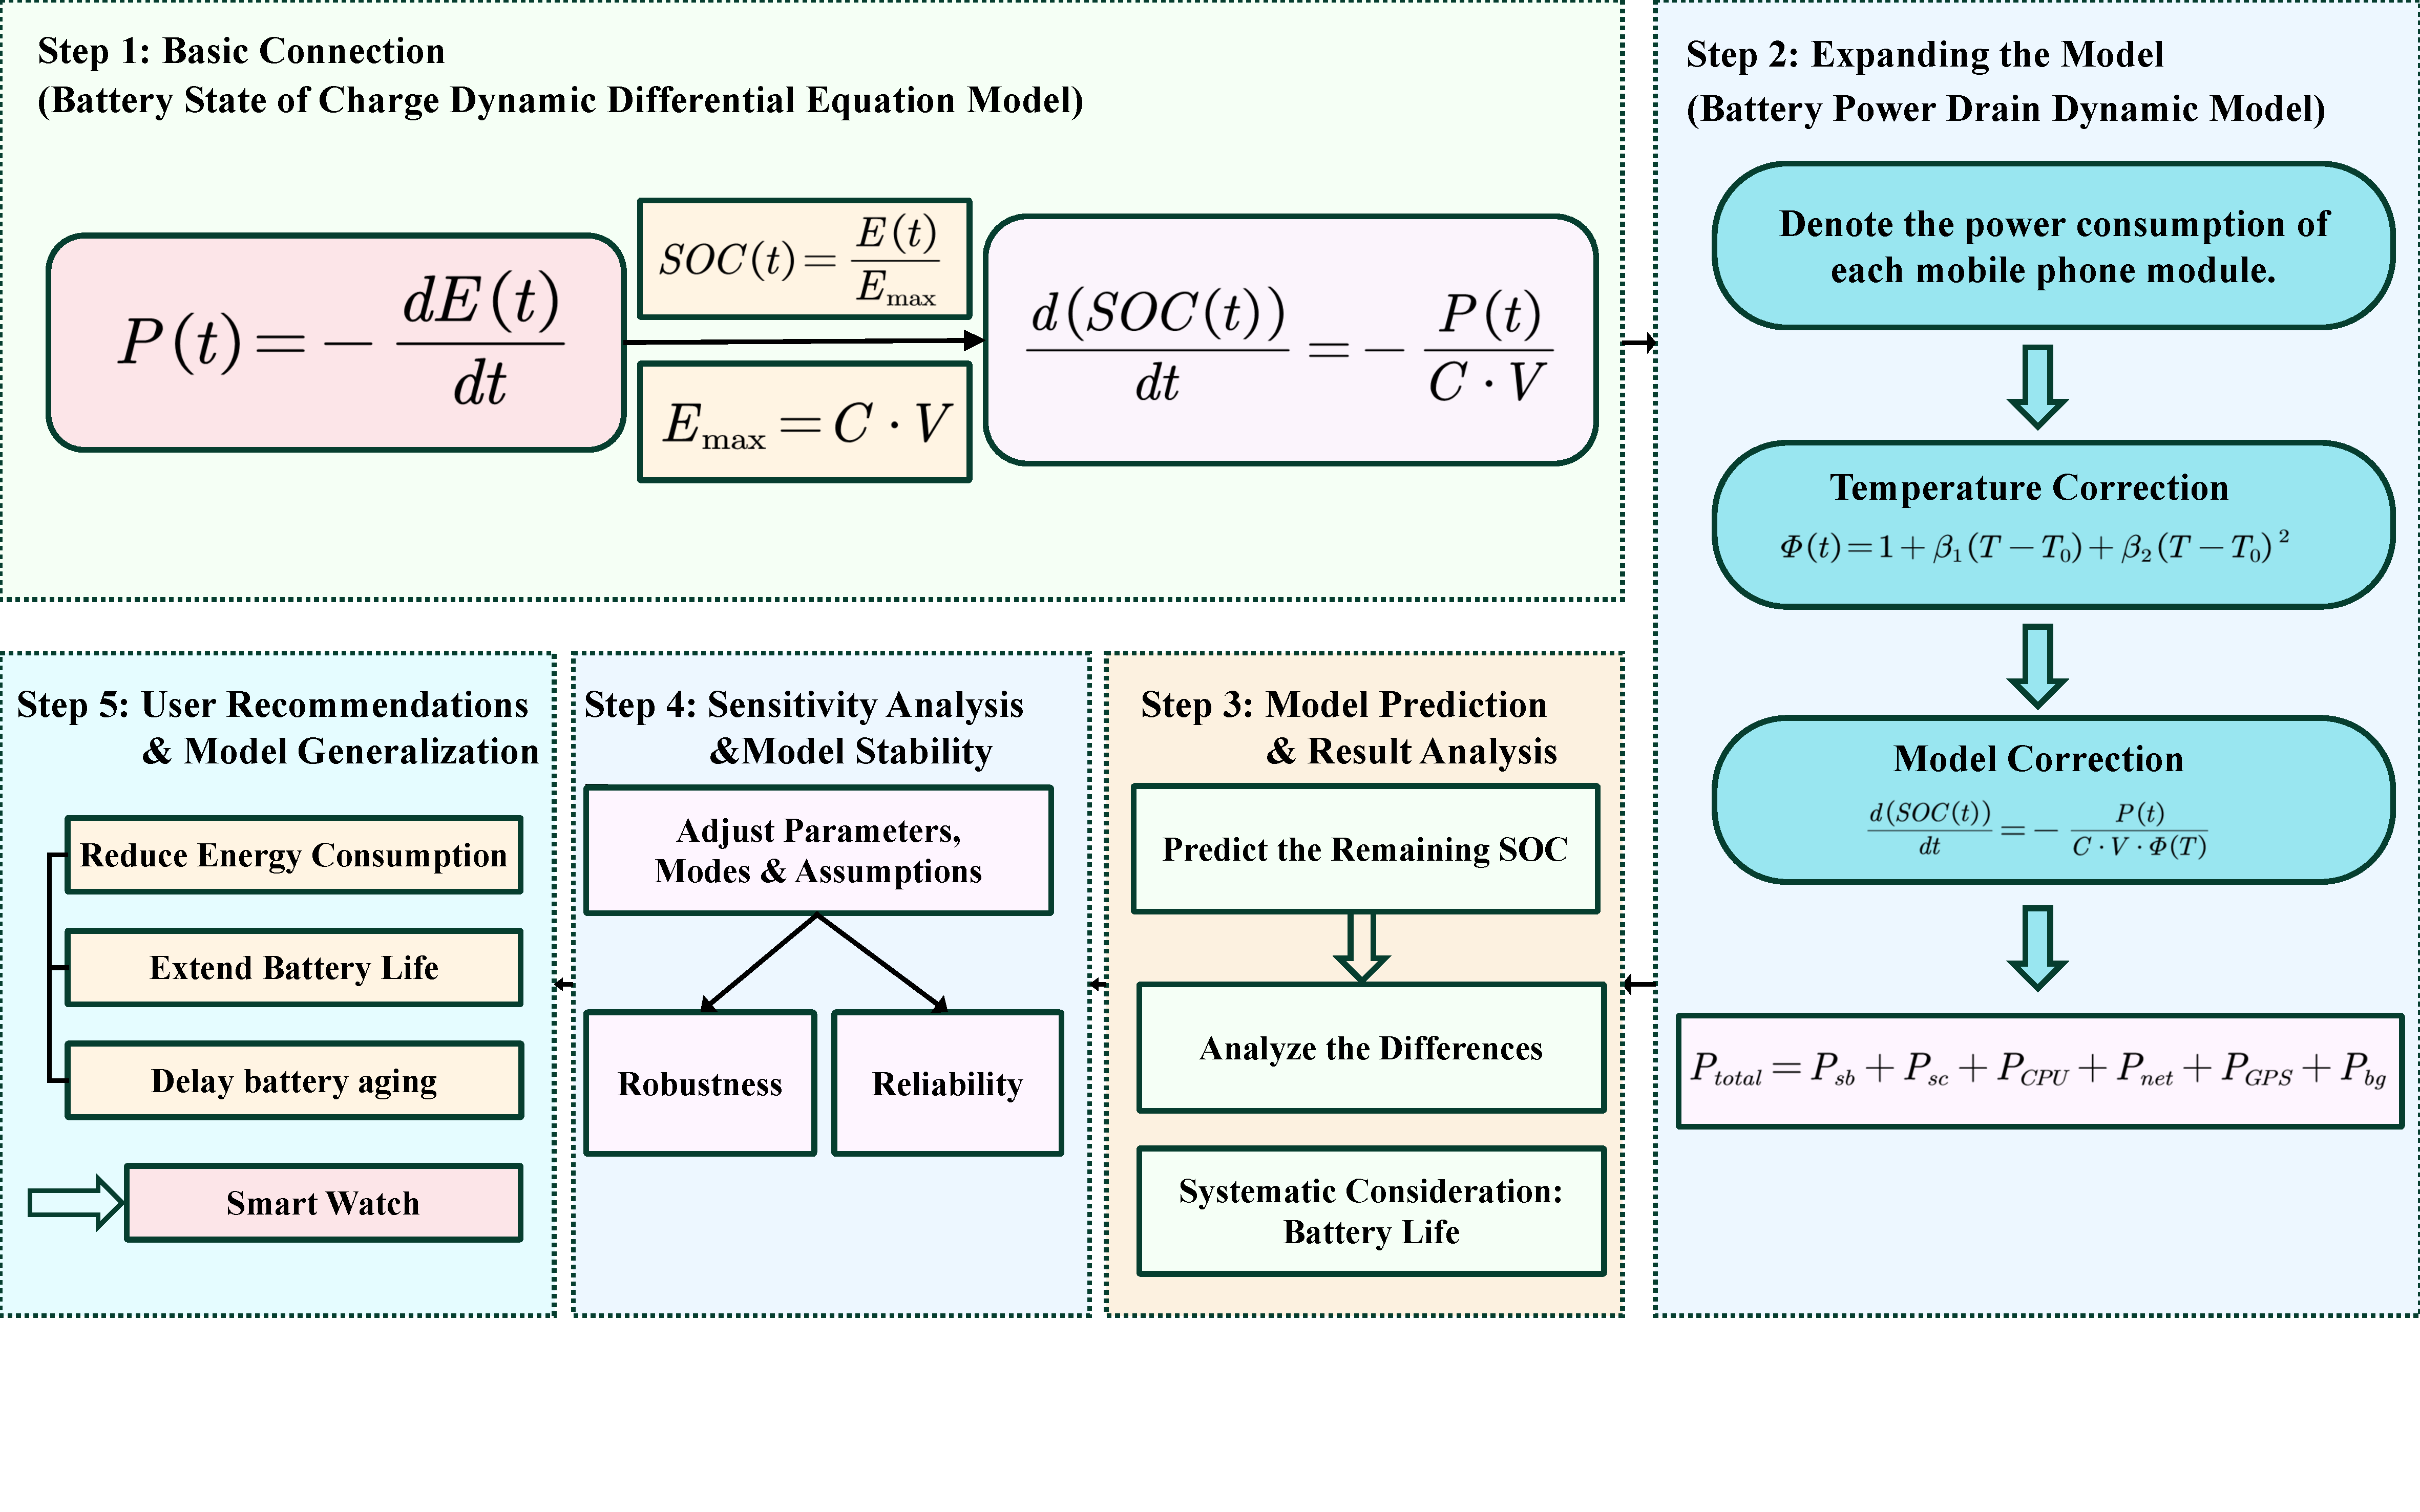
\includegraphics[width=0.55\textwidth]{figures/2026美赛流程图.pdf}
\caption{Y染色体浓度与孕周数的关系散点图}
\label{Y染色体浓度与孕周数的关系散点图}
\end{figure}

\begin{figure}[ht]
\centering
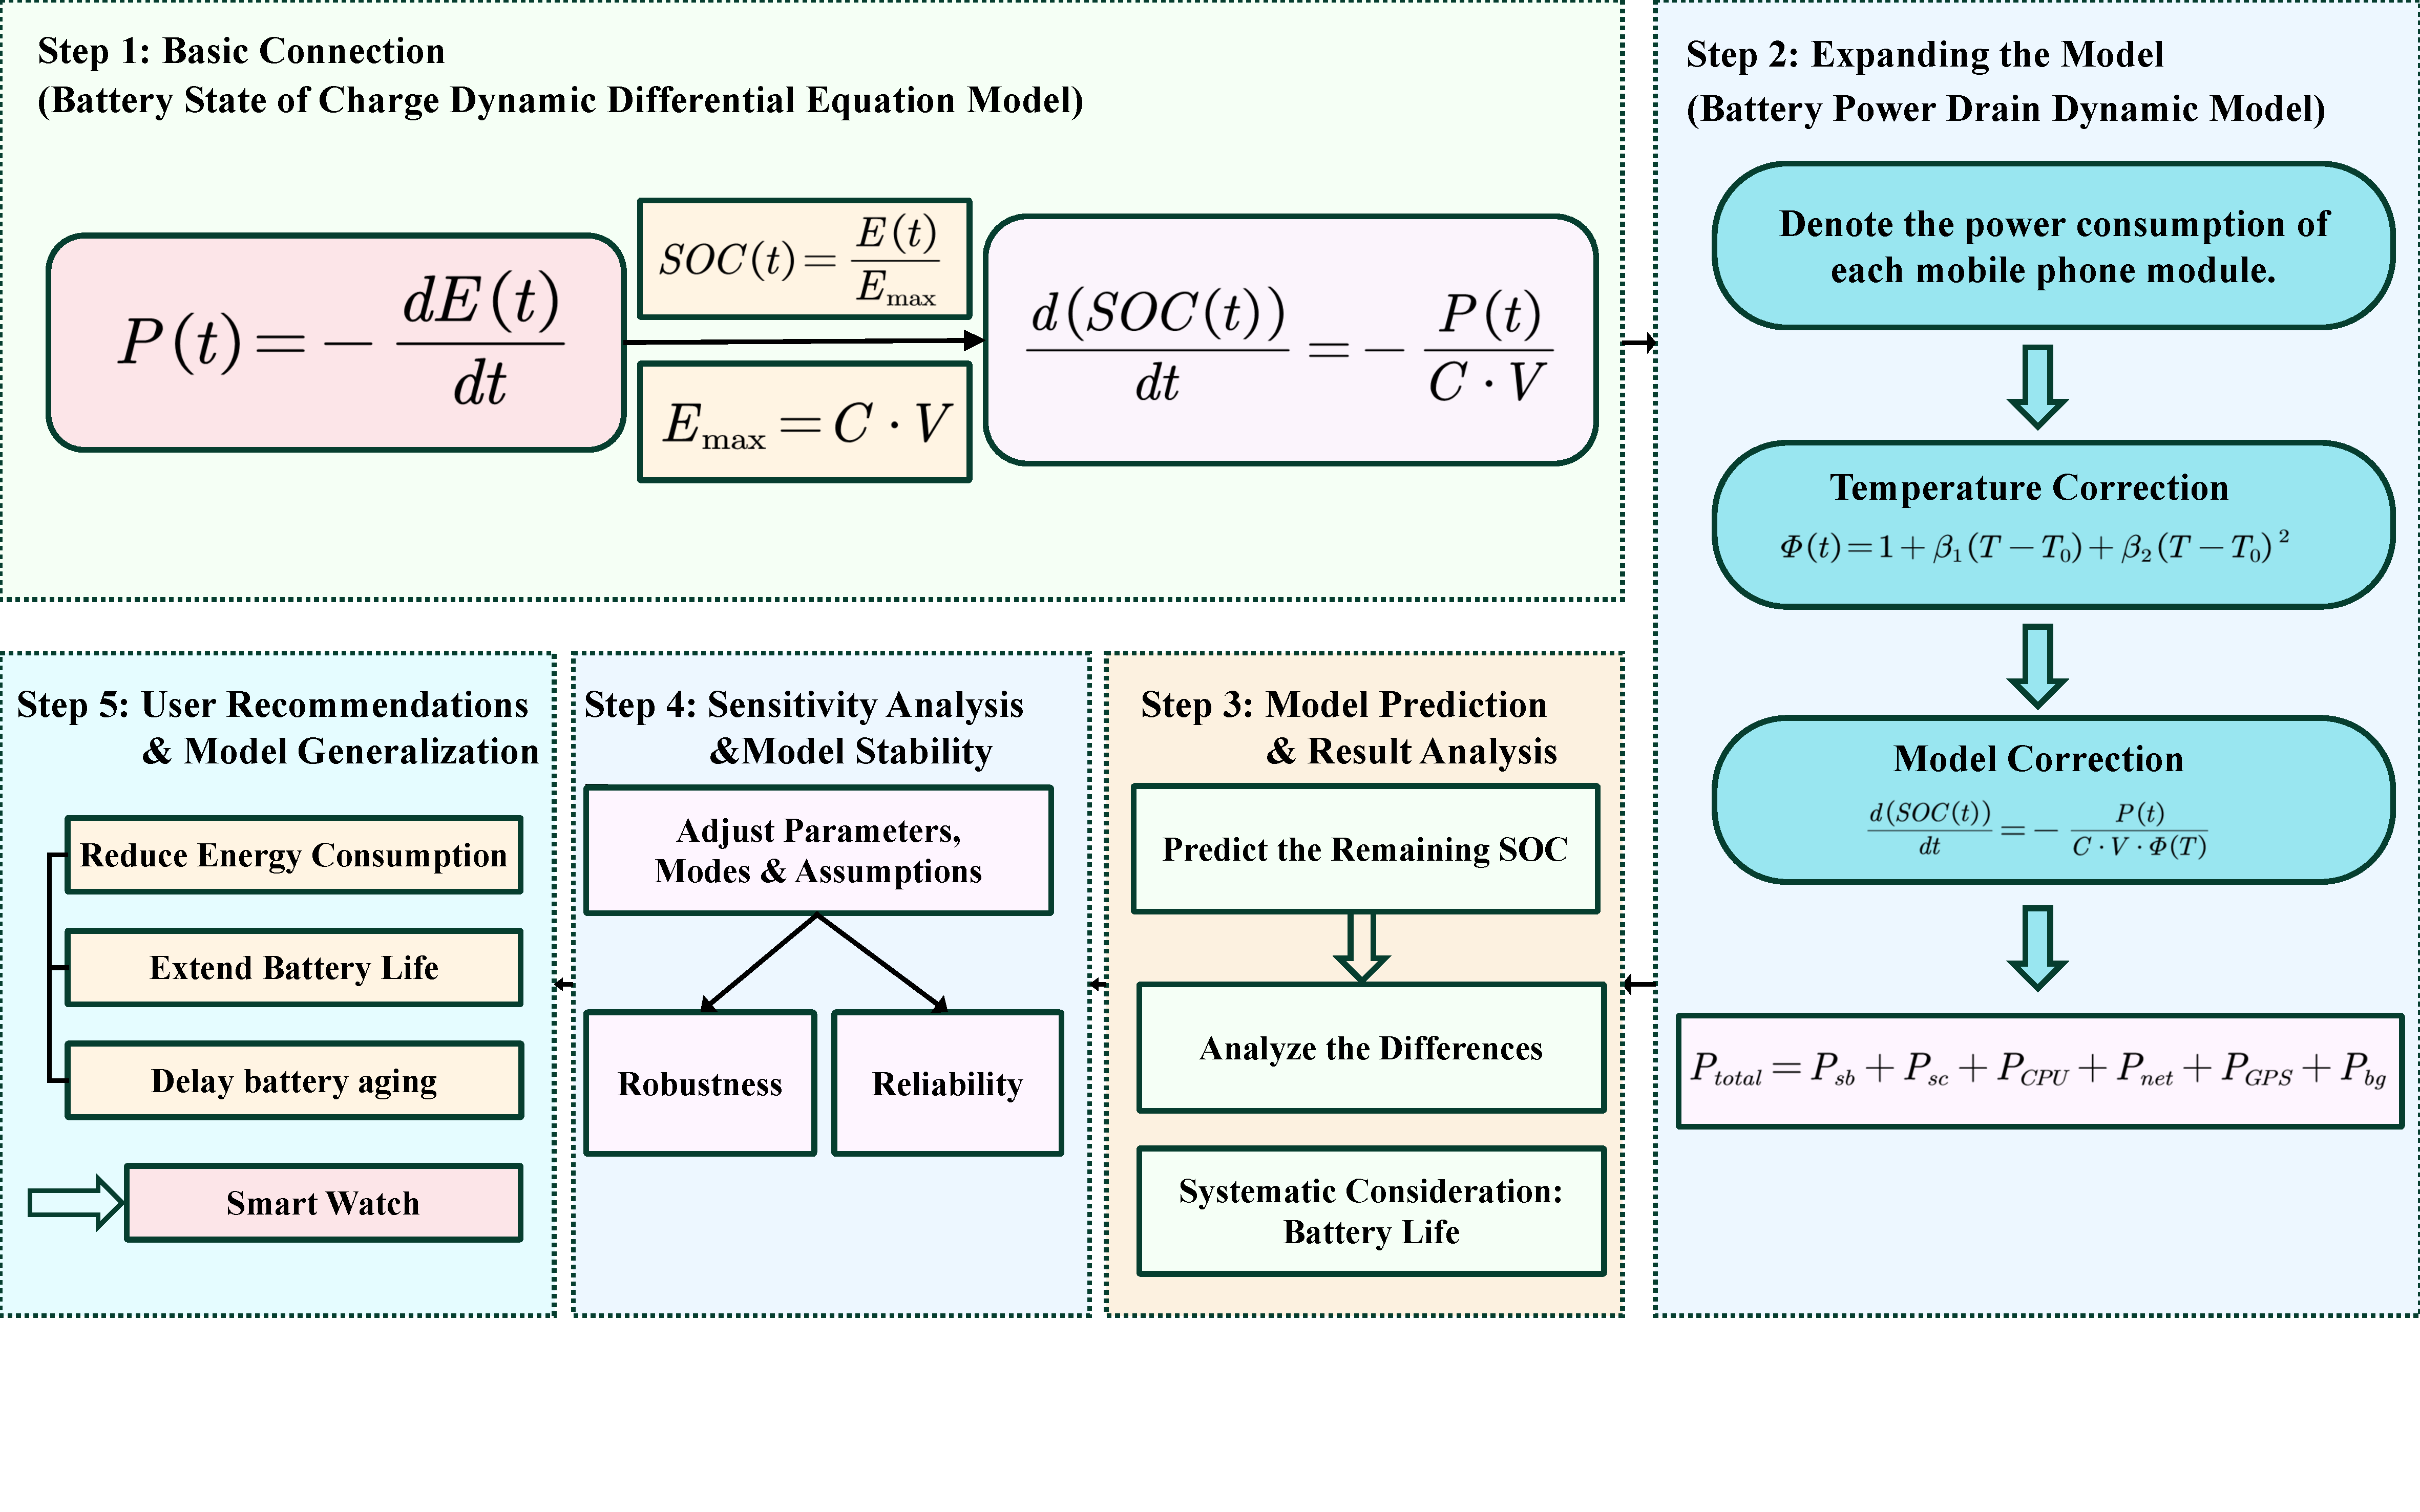
\includegraphics[width=0.55\textwidth,trim=0cm 6.5cm 0cm 0cm, 
clip]{figures/2026美赛流程图.pdf}
\label{Y染色体浓度与BMI的关系散点图}
\caption{Y染色体浓度与BMI的关系散点图}
\end{figure}

使用MATLAB求解Y染色体浓度与孕周数、BMI间的Pearson相关系数，并绘制热力图：
\begin{figure}[ht]
\centering
{
\includegraphics[width=.45\textwidth,trim=0cm 6.5cm 0cm 0cm, 
	clip]{2026美赛流程图.pdf}}
{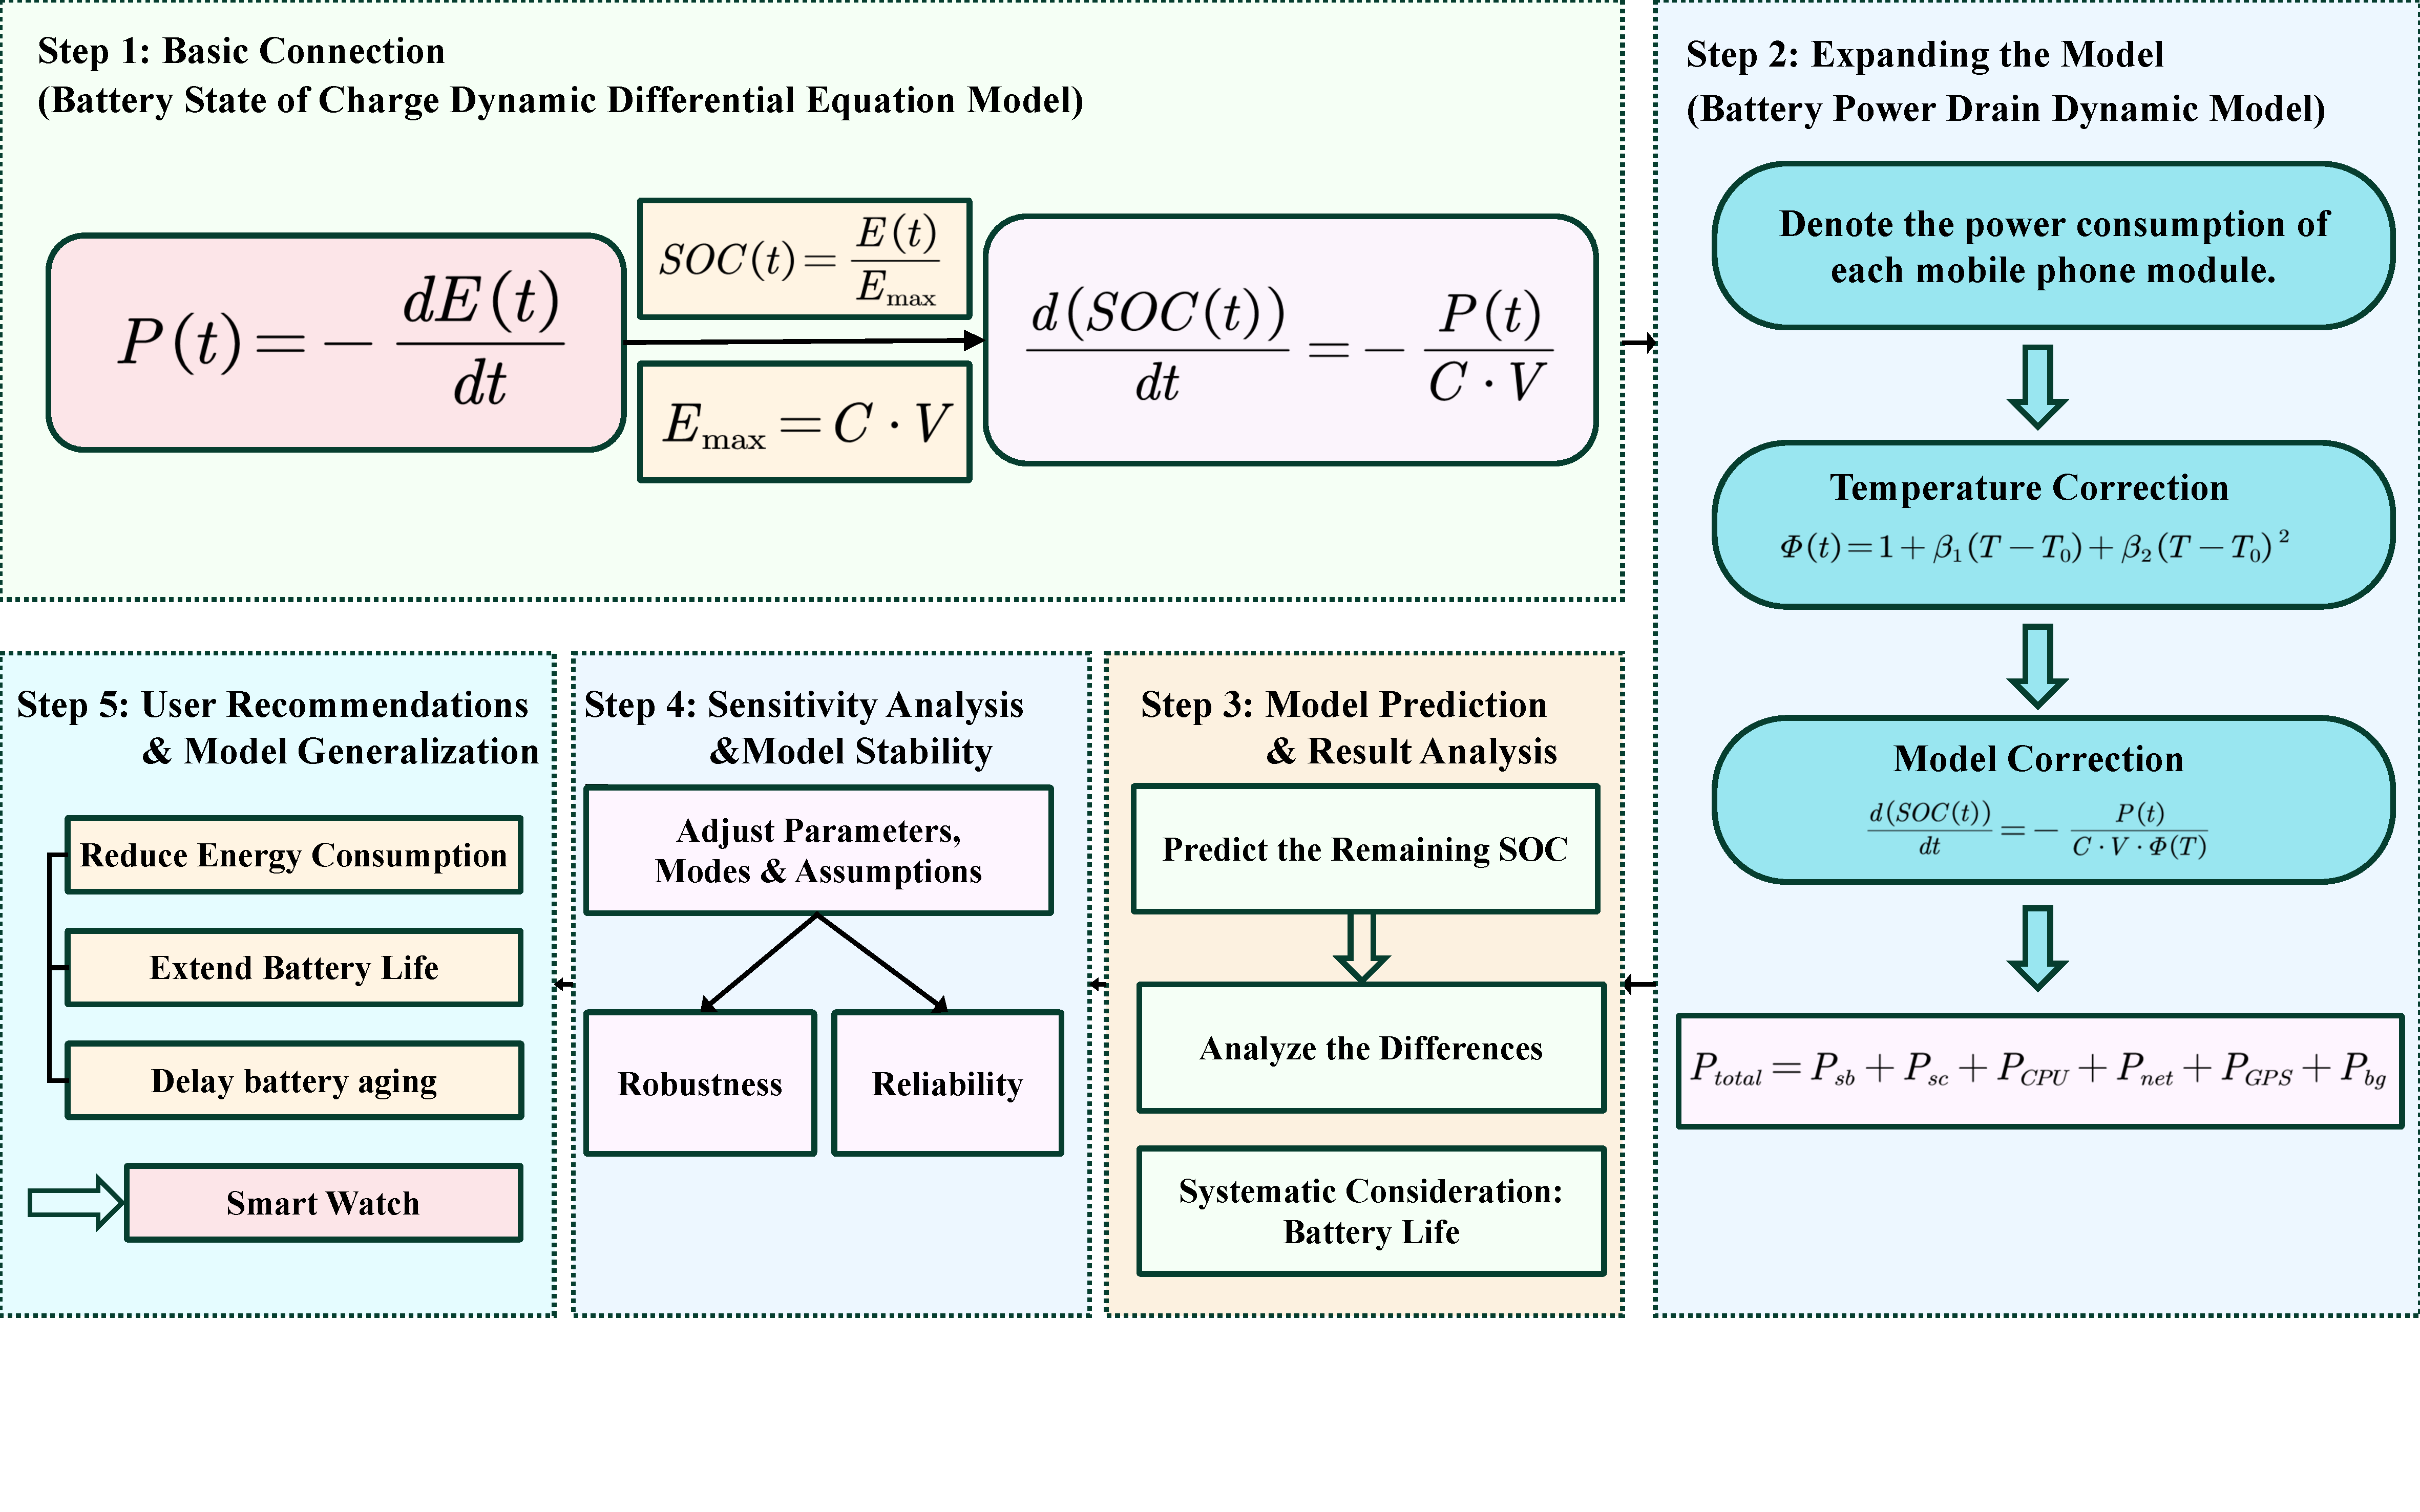
\includegraphics[width=.45\textwidth,trim=0cm 6.5cm 0cm 0cm, 
	clip]{figures/2026美赛流程图.pdf}}
\caption{Y染色体浓度与孕周数、BMI间Pearson相关系数热力图}\label{fig:Y染色体浓度与BMI间Pearson相关系数热力图}
\end{figure}

    \item Pearson相关系数检验
    
    本文对上述结果Pearson相关系数检验，检验步骤如下：
    
    \textbf{Step 1. 提出假设}
    
    原假设 \( H_0 \)：Pearson 相关系数 \( R \neq 0 \)
    
    备择假设 \( H_1 \)：Pearson 相关系数 \( R = 0 \)
    
    设置信水平为 \( 95\% \)
    
    \textbf{Step 2. 计算P值}

本文利用 MATLAB 进行 Pearson 相关系数检验，结果如下表所示：
\begin{table}[H]
\centering
\caption{Y 染色体浓度与孕周数、BMI 的 Pearson 相关系数检验P值}
\renewcommand{\arraystretch}{1.5}
\setlength{\tabcolsep}{2.5em}
\renewcommand{\heavyrulewidth}{1.2pt}
\begin{tabular}{cccc}
\toprule
指标 1 & 指标 2 & \( P \) 值 & 显著性 \\
\midrule
Y 染色体浓度 & 孕周数 & 0.000029796 & *** \\
Y 染色体浓度 & BMI & 0.000000574 & *** \\
\bottomrule
\end{tabular}
\label{tab:pearson_p_value}
\end{table}

\(p < 0.001\)代表关系高度显著，使用***表示，\(p < 0.01\)代表关系非常显著，使用**表示，\(p < 0.05\)代表关系显著，使用*表示，\(p > 0.05\)代表关系不显著，不进行标注。

由表 1 得出，各品类销售量间的 Pearson 相关系数均小于置信水平 0.05，拒绝原假设，所得关系高度显著。
\end{enumerate}	

\subsection{利用Pearson相关系数分析Y染色体浓度与其他指标的相关性}

与\ref{5.1}类似，进行所有指标间的热力图可视化：
\newpage
\begin{figure}[ht]
\centering
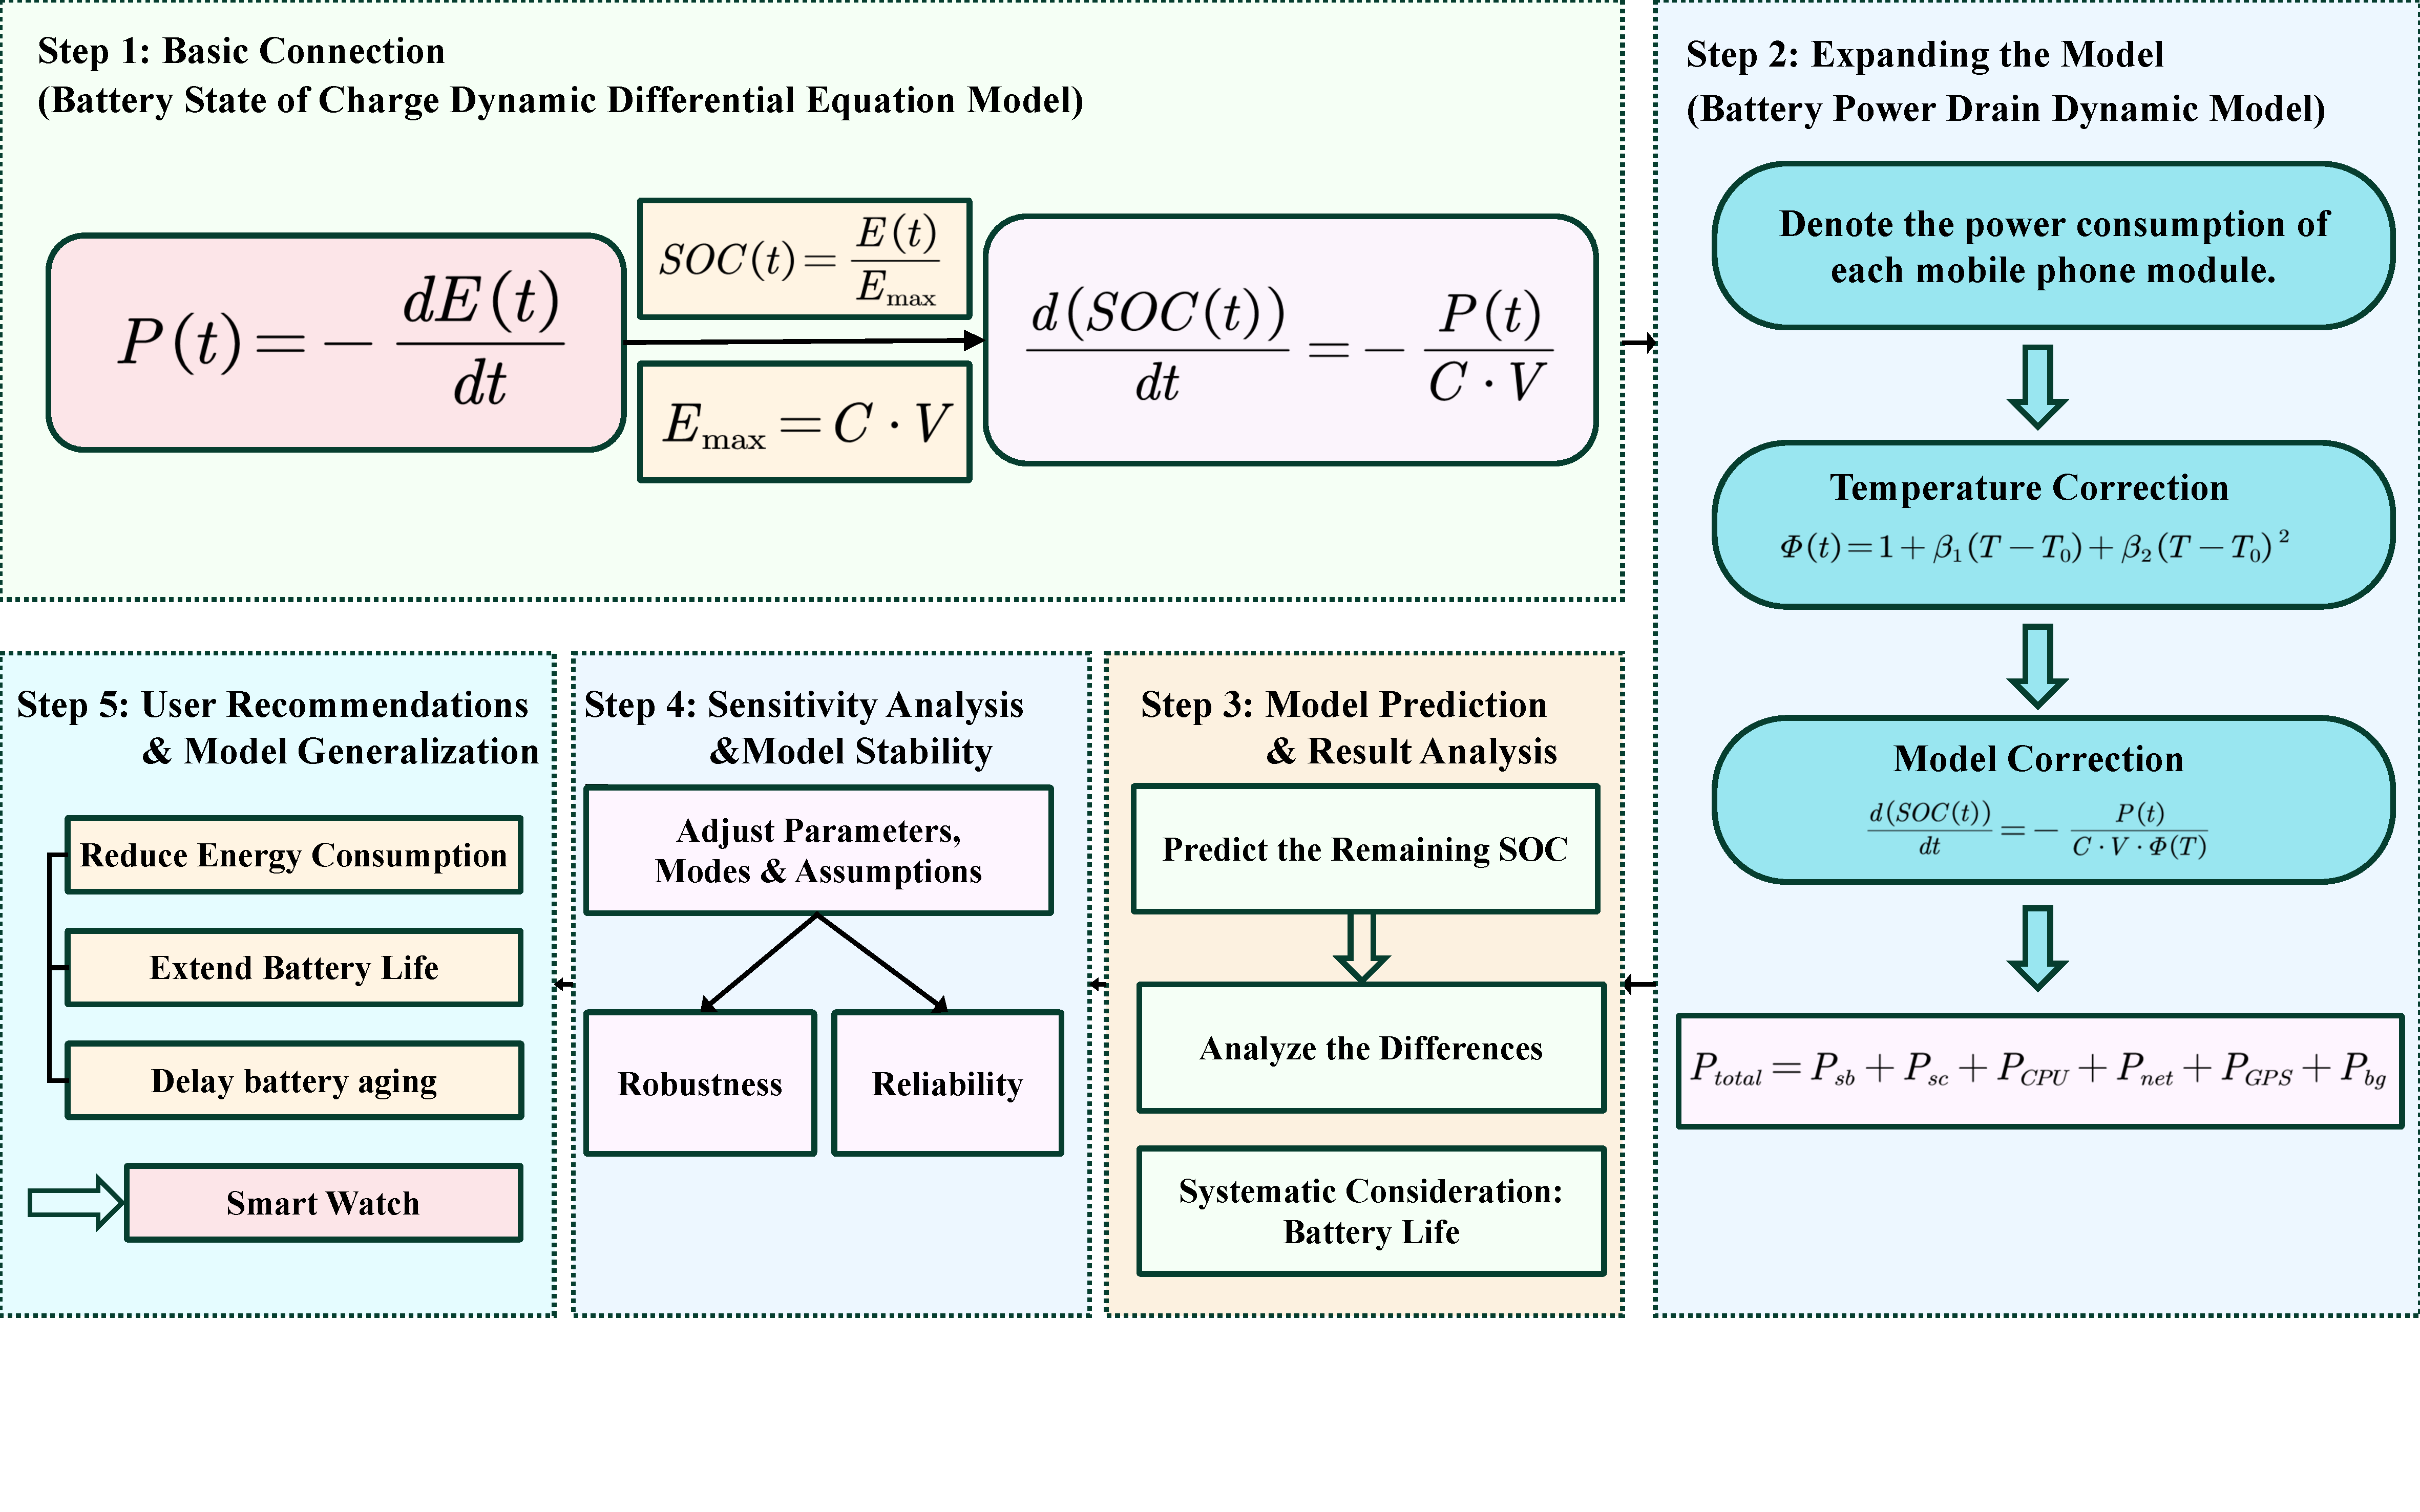
\includegraphics[width=1.05\textwidth,trim=0cm 6.5cm 0cm 0cm, 
clip]{figures/2026美赛流程图.pdf}
\label{fig:所有指标间热力图}
\caption{所有指标间热力图}
\end{figure}

通过热力图可知，以\(R^2=0.4\)为阈值区分较强相关指标与弱相关指标，Y染色体浓度仅与X染色体浓度较强相关，但这并无太大意义，故不继续分析。
\subsection{通过合适的回归方式求解关系方程}

\begin{enumerate}[label=(\arabic*)]
    \item 线性回归
    首先尝试线性回归求解Y染色体浓度与孕周数、BMI的关系方程，对原始数据通过MATLAB直接进行线性回归拟合：
    \begin{figure}[ht]
    \centering
    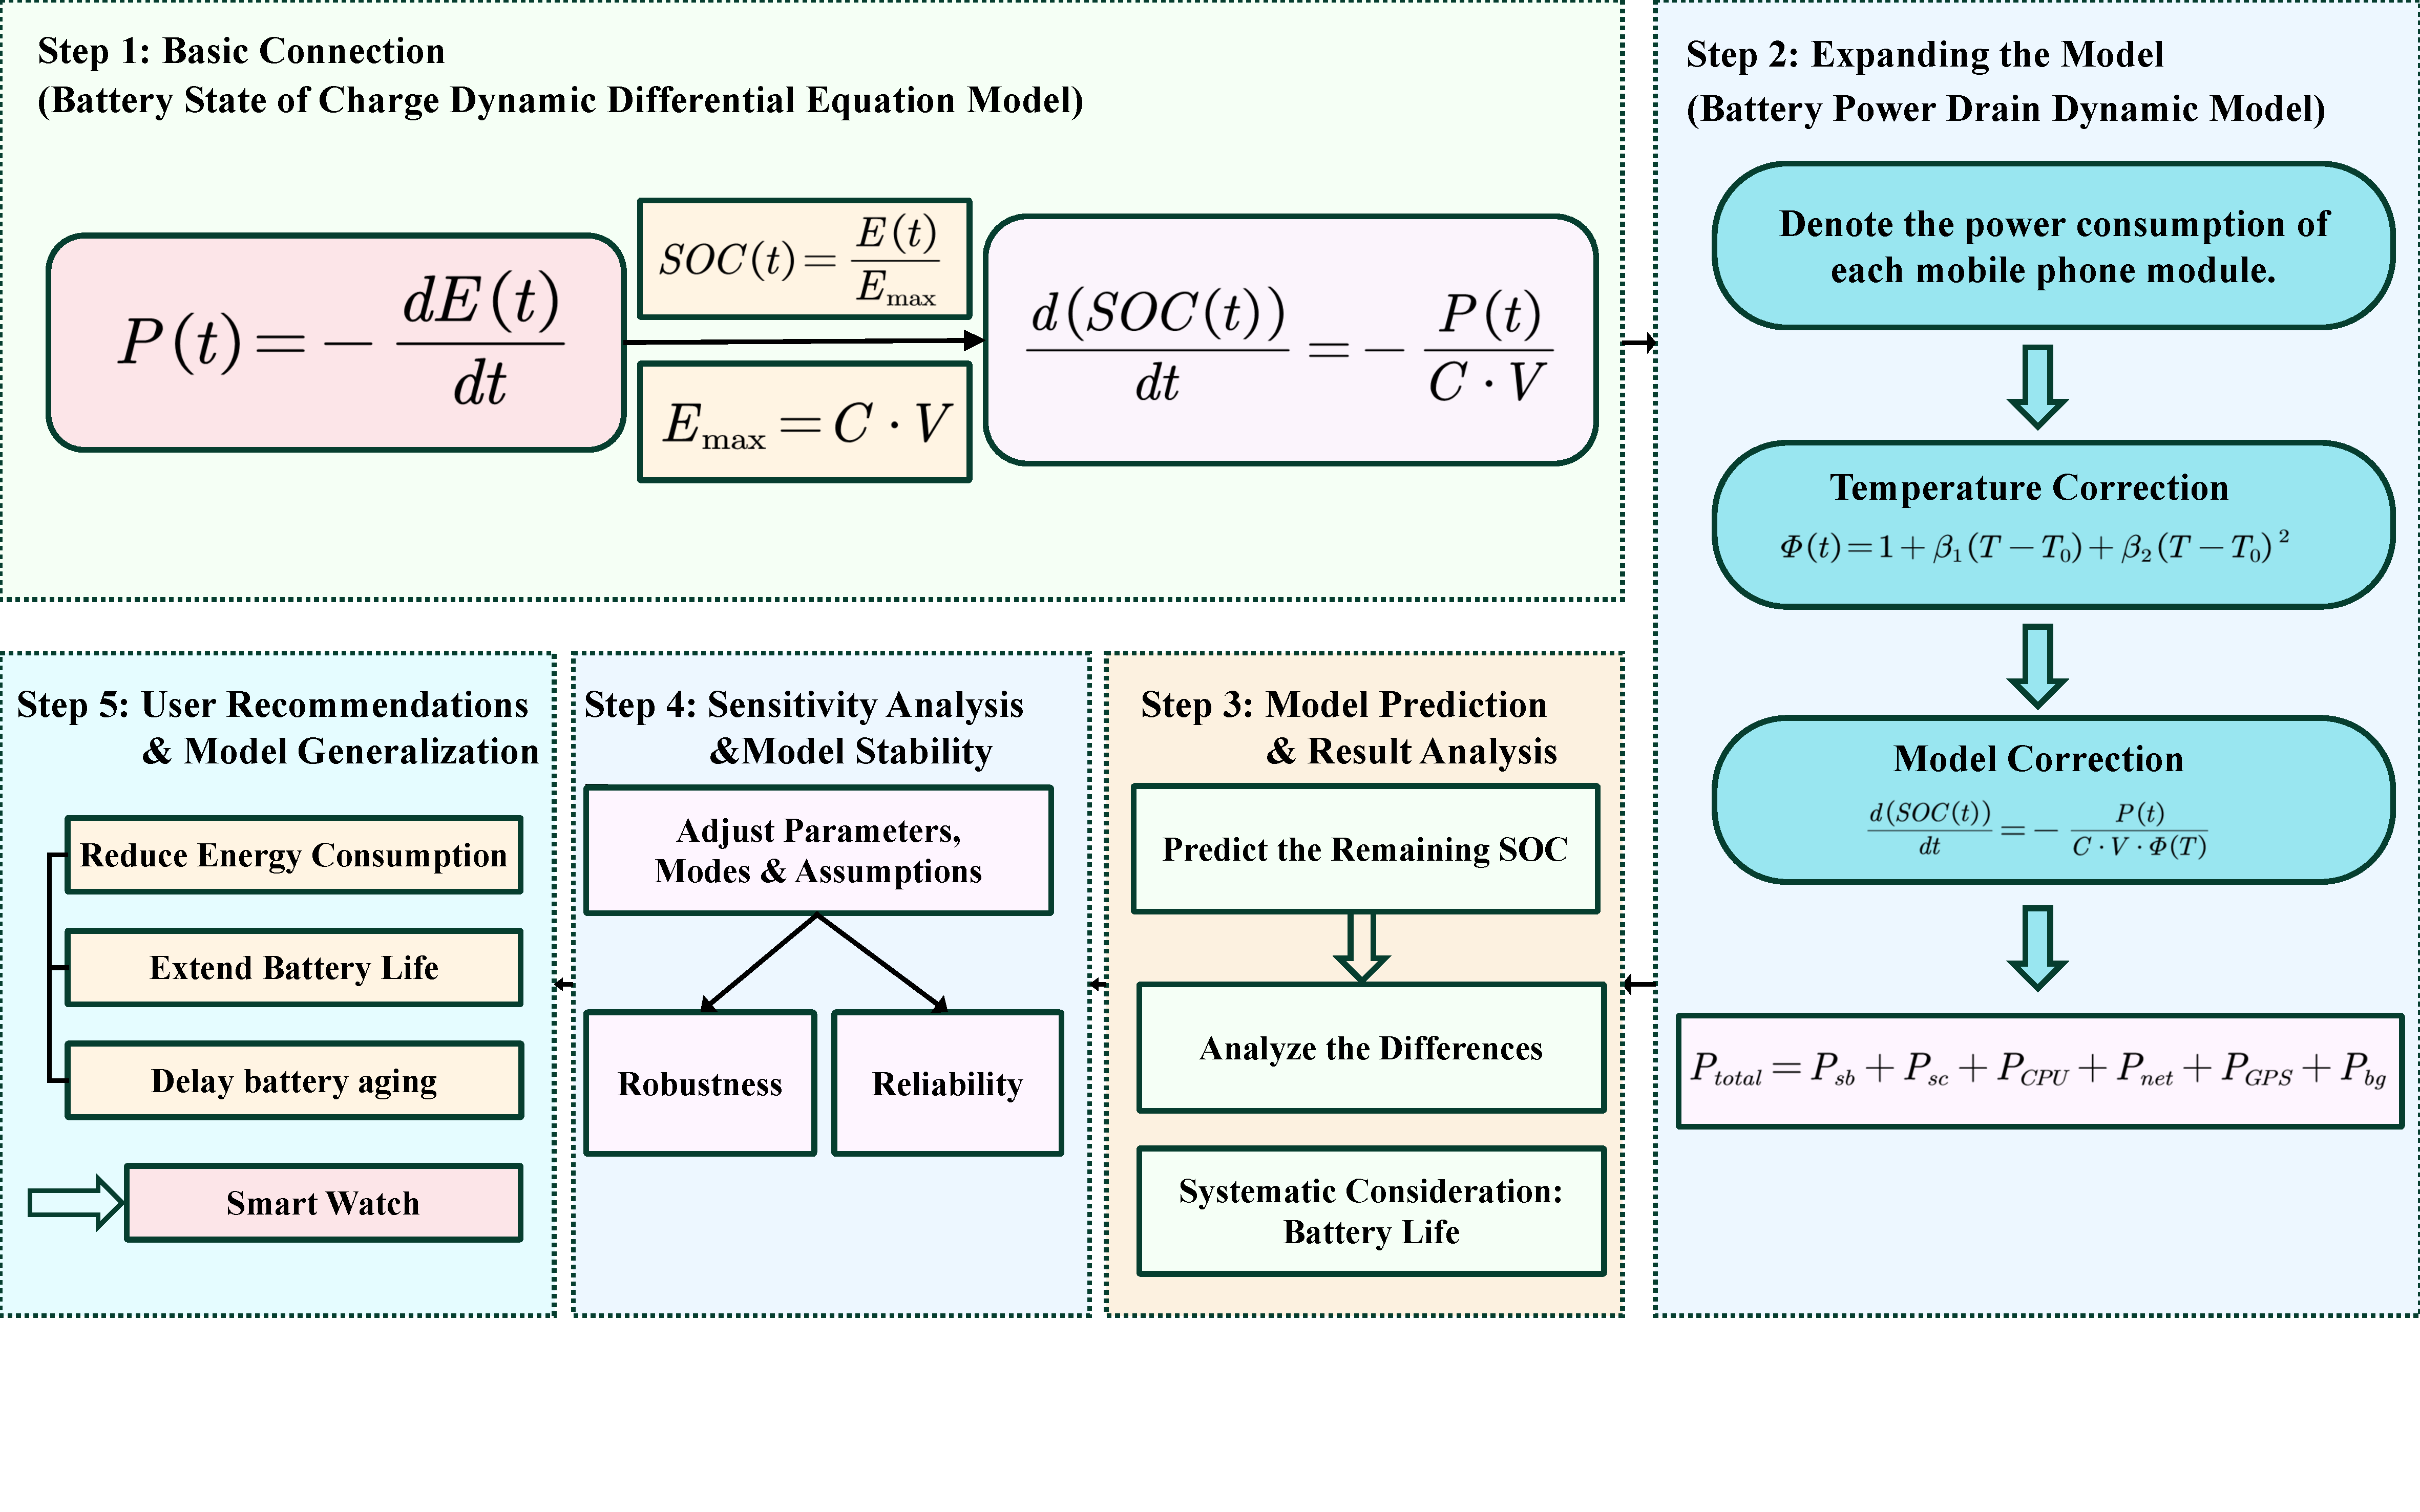
\includegraphics[width=0.95\textwidth,trim=0cm 6.5cm 0cm 0cm, 
    clip]{figures/2026美赛流程图.pdf}
    \label{fig:线性回归Y染色体浓度与孕周数、BMI线性回归拟合图像}
    \caption{线性回归Y染色体浓度与孕周数、BMI线性回归拟合图像}
    \end{figure}

    指标间的相关系数检验结果如下表所示：
    \begin{table}[H]
\centering
\caption{线性回归 Y 染色体浓度与孕周数、BMI 相关系数检验结果}
\renewcommand{\arraystretch}{1.5}
\setlength{\tabcolsep}{3em}
\begin{tabular}{ccc}
\toprule
指标 1 & 指标 2 & \( \text{R}^2 \) \\
\midrule
Y 染色体浓度 & 孕周数 & 0.016 \\
Y 染色体浓度 & BMI & 0.023 \\
\bottomrule
\end{tabular}
\label{tab:linear_regression_r2}
\end{table}

由上表看出，两组指标间相关系数检验结果较差，表明对原数据直接拟合效果不佳，考虑多元线性回归优化拟合效果，综合考虑两种指标影响再次进行线性拟合。
    \item 
\end{enumerate}	











%%%%%%%%%%%%%%%%%%%%%%%%%%%%%%%%%%%%%%%%%%%%%%%%%%%%%%%%%%%%% 

\section{问题二的模型的建立和求解}
\subsection{模型建立}

引用\cref{fig:双图}，引用\cref{fig:双图a}，引用\cref{fig:双图b}。

\begin{figure}[ht]
\centering
\subcaptionbox{双图a子标题\label{fig:双图a}}
{
\includegraphics[width=.4\textwidth]{2026美赛流程图.pdf}}
\subcaptionbox{双图b子标题\label{fig:双图b}}
{
\includegraphics[width=.4\textwidth]{2026美赛流程图.pdf}}
\caption{双图}\label{fig:双图}
\end{figure} 

\subsection{模型求解}

\textbf{Step1：} 

\textbf{Step2：} 

\textbf{Step3：} 

\subsection{求解结果}

%%%%%%%%%%%%%%%%%%%%%%%%%%%%%%%%%%%%%%%%%%%%%%%%%%%%%%%%%%%%% 

\section{问题三的模型的建立和求解}
\subsection{模型建立}

\subsection{模型求解}

\textbf{Step1：} 

\textbf{Step2：} 

\textbf{Step3：} 

\subsection{求解结果}

%%%%%%%%%%%%%%%%%%%%%%%%%%%%%%%%%%%%%%%%%%%%%%%%%%%%%%%%%%%%% 

\section{问题四的模型的建立和求解}
\subsection{模型建立}

\subsection{模型求解}

\textbf{Step1：} 

\textbf{Step2：} 

\textbf{Step3：} 

\subsection{求解结果}

%%%%%%%%%%%%%%%%%%%%%%%%%%%%%%%%%%%%%%%%%%%%%%%%%%%%%%%%%%%%%

\section{模型的分析与检验}

\subsection{灵敏度分析}

\subsection{误差分析}

%%%%%%%%%%%%%%%%%%%%%%%%%%%%%%%%%%%%%%%%%%%%%%%%%%%%%%%%%%%%%

\section{模型的评价}

\subsection{模型的优点}
\begin{itemize}[itemindent=2em]
\item 优点1
\item 优点2
\item 优点3
\end{itemize}

\subsection{模型的缺点}
\begin{itemize}[itemindent=2em]
\item 缺点1
\item 缺点2
\end{itemize}

%%%%%%%%%%%%%%%%%%%%%%%%%%%%%%%%%%%%%%%%%%%%%%%%%%%%%%%%%%%%%
%% 参考文献
\nocite{*}
\begin{thebibliography}{9}%宽度9
\bibitem{1} 边旭明.胎儿染色体非整倍体的无创DNA产前检测[J].实用妇产科杂志,2013,29(05):330-333.
\bibitem{2} 罗潇.法律规制视野下的当代中国生育行为研究[D].西南财经大学,2014.
\bibitem{3} EHRICH M, DECIU C, ZWIEFELHOFER T, 等. Noninvasive detection of fetal trisomy 21 by sequencing of DNA in maternal blood: a study in a clinical setting[J/OL]. American Journal of Obstetrics and Gynecology, 2011, 204(3): 205.e1-205.e11. DOI:10.1016/j.ajog.2010.12.060.
\bibitem{4} 徐勇勇,陈长生,曹秀堂,等.医学与卫生统计资料的系统结构数据[Ｊ].中国卫生统计,1995,12(5)：12-15.
\bibitem{4}徐勇勇,陈长生,曹秀堂,等.医学与卫生统计资料的系统结构数据[Ｊ].中国卫生统计,1995,12(5)：12-15.
\bibitem{5}余松林.混合线性模型的应用[J].中国医院统计,2006,(01):70-75.
\bibitem{6}毛典辉.基于MapReduce的Canopy-Kmeans改进算法[J].计算机工程与应用,2012,48(27):22-26+68.
\bibitem{7}DeepSeek Chat, DeepSeek-V3, 深度求索（DeepSeek）, 2025-09-05.
\bibitem{8}龙文佳,张晓峰,张链.基于k-means和肘部法则的业务流程聚类方法[J].江汉大学学报(自然科学版),2020,48(01):81-90.DOI:10.16389/j.cnki.cn42-1737/n.2020.01.011.
\bibitem{9}DeepSeek Chat, DeepSeek-V3, 深度求索（DeepSeek）, 2025-09-05.
\bibitem{10}DeepSeek Chat, DeepSeek-V3, 深度求索（DeepSeek）, 2025-09-06.
\bibitem{11}栾丽华,吉根林.决策树分类技术研究[J].计算机工程,2004,(09):94-96+105
\bibitem{12}李琪,张欣,张平康,等.基于密度峰值优化的Canopy-Kmeans并行算法[J].通信技术,2018,51(02):312-317.
\end{thebibliography}
\newpage
%%%%%%%%%%%%%%%%%%%%%%%%%%%%%%%%%%%%%%%%%%%%%%%%%%%%%%%%%%%%%
%% 附录
\begin{appendices}
\section{文件列表}
\begin{table}[H]
\centering
\begin{tabularx}{\textwidth}{LC}
\toprule
文件名   & 功能描述 \\
\midrule
q1.m & 问题一程序代码 \\
q2.py & 问题二程序代码 \\
q3.c & 问题三程序代码 \\
q4.cpp & 问题四程序代码 \\
\bottomrule
\end{tabularx}
\label{tab:文件列表}
\end{table}

\section{代码}
\noindent Q1\_1scatter\_therm.m
\lstinputlisting[language=matlab]{code/Q1_1scatter_therm.m}
q2.py
\lstinputlisting[language=python]{code/q2.py}
q3.c
\lstinputlisting[language=c]{code/q3.c}
q4.cpp
\lstinputlisting[language=c++]{code/q4.cpp}
\end{appendices}
\end{document}


